\documentclass[a4paper,12pt]{article}

\usepackage[T2A]{fontenc}
\usepackage[utf8]{inputenc}
\usepackage[russian]{babel}

\usepackage[margin=2cm]{geometry}
\usepackage{amsmath, amssymb}

\usepackage{graphicx}
\graphicspath{{assets}}

\usepackage{array}
\usepackage{float}
\usepackage{longtable}
\usepackage{multirow}
\usepackage{setspace}

\usepackage{hyperref}
\hypersetup{%
    colorlinks=true,
    linkcolor=blue,
    filecolor=magenta,
    urlcolor=magenta,
}

\setlength{\parindent}{0pt}

\newcommand\Section[1]{%
\refstepcounter{section}%
\section*{%
\raggedright
\arabic{section}. #1
}%
\addcontentsline{toc}{section}{\arabic{section}. #1}%
}

\newcommand\Subsection[1]{%
\refstepcounter{subsection}%
\subsection*{%
\raggedright%
\arabic{section}. \arabic{subsection}. #1
}%
\addcontentsline{toc}{subsection}{\arabic{subsection}. #1}%
}

\begin{document}

% ---------- HEADER ----------

\begin{minipage}{0.55\textwidth}
    \begin{center}
        \textbf{Университет ИТМО}\\
        Физико-технический факультет\\
        Физический факультет
    \end{center}
\end{minipage}
\hfill
\begin{minipage}{0.35\textwidth}
    \begin{flushright}
        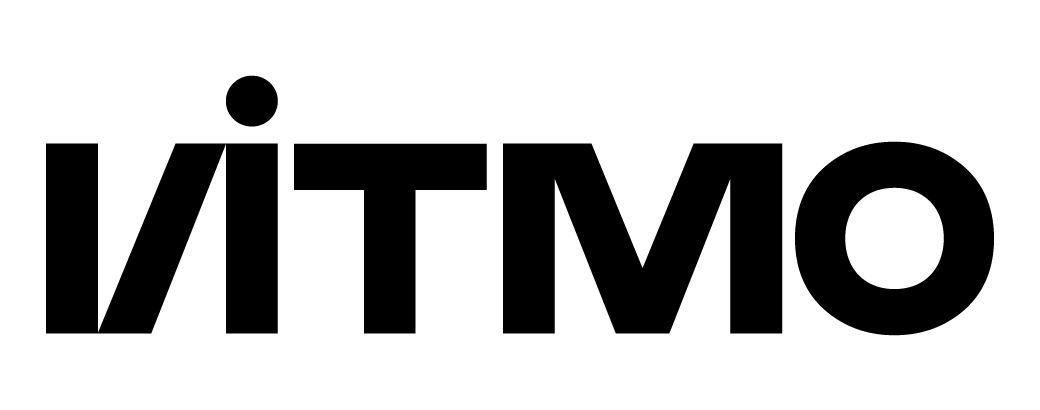
\includegraphics[width=3.2cm]{assets/itmo_logo.png}
    \end{flushright}
\end{minipage}

\vspace{1.2cm}

\begin{tabular}{@{}p{7cm}p{6cm}@{}}
Группа\hspace{0.3cm}%
\makebox[4cm]{\rlap{\raisebox{0.3ex}{\hspace{1.0cm}ПИИКТ 2.2}}\hrulefill}
&
К работе допущен \hrulefill
\\[0.8cm]
Студент\hspace{0.3cm}%
\makebox[4cm]{\rlap{\raisebox{0.3ex}{\hspace{0.5cm}Бых Д. М.}}\hrulefill}
&
Работа выполнена \hrulefill
\\[0.8cm]
Преподаватель\hspace{0.2cm}%
\makebox[3cm]{\rlap{\raisebox{0.3ex}{\hspace{0.5cm}Рудель А. Е.}}\hrulefill}
&
Отчет принят \hrulefill
\end{tabular}

\vspace{1.2cm}

\begin{center}
{\Large\bfseries Рабочий протокол и отчет по\\ лабораторной работе №1.09}
\vspace{1cm}

{\large \textit{Определение момента инерции методом крутильных колебаний}}
\end{center}

\vspace{2cm}

\Section{Цель работы}
Определение моментов инерции твёрдых тел методом крутильных колебаний и проверка справедливости теоремы Гюйгенса–Штейнера.

\Section{Задачи, решаемые при выполнении работы}
\begin{enumerate}
    \item Измерить массу и геометрические размеры тел различной формы.
    \item Измерить коэффициент угловой жёсткости спиральной пружины.
    \item Измерить периоды крутильных колебаний тел различной формы.
    \item Рассчитать моменты инерции тел различной формы.
    \item Сравнить полученные результаты с теоретическими значениями.
\end{enumerate}

\Section{Объект исследования}
Спиральная пружина, стержень без грузов и с двумя симметрично расположенными грузами, шар и диск с отверстиями. Отдельные цилиндры не исследовались.

\Section{Метод экспериментального исследования}
Угловая жёсткость определяется статическим методом — по зависимости момента внешней силы от угла закручивания. Момент инерции определяется динамическим методом — по периоду свободных крутильных колебаний. Для диска изменяется положение оси относительно центра масс (проверка теоремы Гюйгенса–Штейнера).

\Section{Рабочие формулы и исходные данные}

Основное уравнение динамики вращательного движения:
\[
M = I\varepsilon,\qquad M = -k\varphi,\qquad \frac{d^2\varphi}{dt^2} + \frac{k}{I}\,\varphi = 0,
\]
где $k$ — коэффициент угловой жёсткости пружины, $I$ — момент инерции.

Период крутильных колебаний:
\[
T = 2\pi\sqrt{\frac{I}{k}} \qquad\Longrightarrow\qquad I = \frac{kT^2}{4\pi^2}.
\]

Коэффициент угловой жёсткости (статический метод):
\[
k = \left|\frac{M}{\varphi}\right| = \frac{1}{3}\sum_{i=1}^{3}\frac{|F_i|r_i}{|\varphi|}.
\]

Теорема Гюйгенса–Штейнера и моменты инерции:
\[
I = I_c + m\ell^2,\qquad
I_{\text{ст}} = \frac{mL^2}{12},\qquad
I_{\text{ш}} = \frac{2mR^2}{5},\qquad
I_{\text{д}} = \frac{mR^2}{2},
\]
\[
I_{\text{гр}} = m\!\left(\frac{R^2}{4} + \frac{h^2}{12}\right).
\]

Погрешности (МНК-оценки через стандартные ошибки коэффициентов):
\[
\Delta k = 2s_k = 2\,\frac{s}{\sqrt{\sum(\varphi_i-\bar\varphi)^2}},\qquad
s = \sqrt{\frac{\sum d_i^2}{n-2}},
\]
\[
\Delta I = I\sqrt{\left(\frac{\Delta k}{k}\right)^2 + \left(\frac{2\Delta T}{T}\right)^2},\qquad
\Delta T = \frac{T_{\max} - T_{\min}}{2}.
\]

\noindent\textbf{Исходные данные (массы и размеры, $m$ в кг, размеры в м):}\\
Шар: $m = 0.883$, $D = 0.159$, $R = 0.0795$;\\
Диск с отверстиями: $m = 0.397$, $D = 0.297$, $R = 0.1485$;\\
Стержень: $m = 0.172$, $L = 0.599$;\\
Каждый из двух грузов: $m = 0.231$, $D = 0.031$, $R = 0.0155$, $h = 0.041$, $\ell \approx 0.048$;\\
Плечи приложения силы динамометра: $r_1 = 0.28$, $r_2 = 0.20$, $r_3 = 0.10$ м;\\
Шаг отверстий диска принят $0.030$ м (по данным установки); положения $\ell = 0$; $0.030$; $0.060$ м.

\Section{Измерительные приборы}
\begin{table}[H]
    \centering
    \renewcommand{\arraystretch}{1.4}
    \begin{tabular}{|c|p{4.5cm}|p{2.5cm}|p{3cm}|p{2.5cm}|}
        \hline
        \textit{№} & \textit{Наименование} & \textit{Тип} & \textit{Диапазон} & \textit{Погрешность} \\
        \hline
        1 & Динамометр & электронный & $-5\ldots+5$ Н & $\pm 0.01$ Н \\
        \hline
        2 & Рулетка & механическая & $0\ldots 1.5$ м & $\pm 1$ мм \\
        \hline
        3 & Весы & лабораторные & до $1000$ г & $\pm 0.5$ г \\
        \hline
        4 & Цифровой счётчик периода & цифровой & до $100$ с & $\pm 0.01$ с \\
        \hline
    \end{tabular}
\end{table}

\Section{Схема установки}
\begin{figure}[H]
    \centering
    \fbox{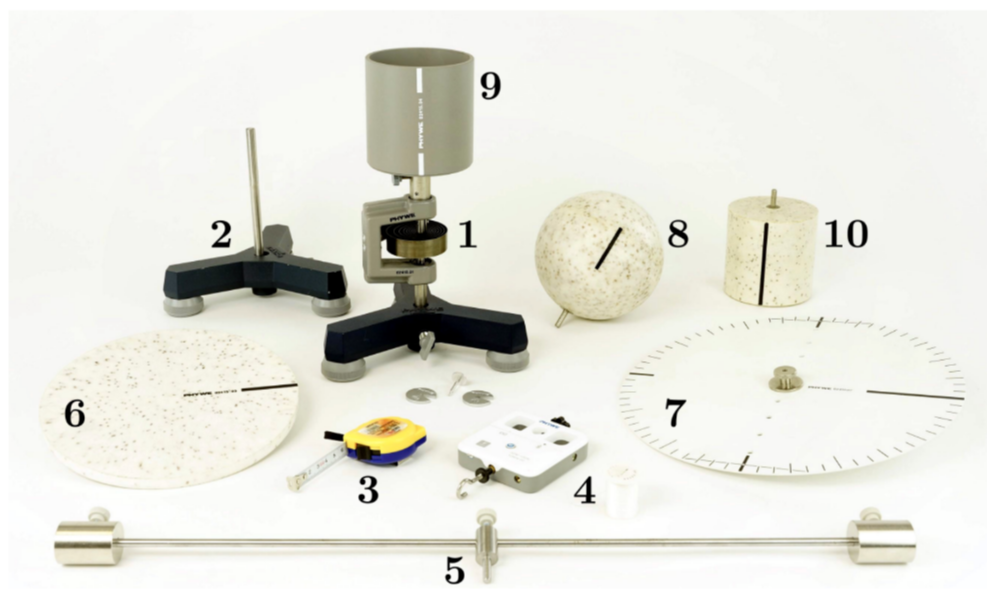
\includegraphics[width=0.75\textwidth]{assets/scheme_1_09.png}}
    \caption{Состав экспериментального стенда (спиральная пружина, динамометр, штанга с грузами, шар, диск)}
    \label{fig:scheme}
\end{figure}

\Section{Результаты прямых измерений}

\Subsection{Определение коэффициента угловой жёсткости}
Показания динамометра снимались при трёх плечах $r_1, r_2, r_3$. Момент силы вычислялся как $M = \frac{1}{3}\sum |F_i|\,r_i$; знак момента задаётся знаком угла закручивания. В таблицу добавлена точка $M(0) = 0$.

\begin{table}[H]
    \centering
    \caption{Момент силы при различных углах закручивания}
    \begin{tabular}{|c|c|c|c|c|c|}
        \hline
        $\varphi$, $^\circ$ & $\varphi$, рад & $F_1$, Н & $F_2$, Н & $F_3$, Н & $\langle M\rangle$, Н$\cdot$м \\
        \hline
        270  & $3\pi/2$   & $0.215$  & $0.345$  & $1.520$ & $9.37\cdot10^{-2}$ \\
        \hline
        180  & $\pi$      & $-0.255$ & $-0.190$ & $-0.315$ & $4.70\cdot10^{-2}$ \\
        \hline
        90   & $\pi/2$    & $-0.465$ & $-0.445$ & $-0.420$ & $8.71\cdot10^{-2}$ \\
        \hline
        $-90$  & $-\pi/2$  & $-0.240$ & $-0.170$ & $0.145$  & $-3.86\cdot10^{-2}$ \\
        \hline
        $-180$ & $-\pi$    & $-0.015$ & $0.145$  & $0.665$  & $-3.32\cdot10^{-2}$ \\
        \hline
        $-270$ & $-3\pi/2$ & $0.155$  & $0.375$  & $0.965$  & $-7.16\cdot10^{-2}$ \\
        \hline
    \end{tabular}
\end{table}

Пример расчёта для $\varphi = 270^\circ$:
\[
\langle M\rangle = \frac{0.215\cdot 0.28 + 0.345\cdot 0.20 + 1.520\cdot 0.10}{3}
= \frac{0.2812}{3} = 9.37\cdot10^{-2}\ \text{Н}\cdot\text{м}.
\]

\Subsection{Измерение периодов колебаний}
Измерялось время $\tau$ трёх полных колебаний; период $T = \tau/3$.

\begin{table}[H]
    \centering
    \caption{Периоды колебаний для исследуемых тел}
    \begin{tabular}{|l|c|c|c|c|c|}
        \hline
        Тело & $\tau_1$, с & $\tau_2$, с & $\tau_3$, с & $\langle T\rangle$, с & $\Delta T$, с \\
        \hline
        Стержень & 7.25 & 7.28 & 7.22 & 2.417 & 0.010 \\
        \hline
        Стержень + 2 груза ($\ell \approx 0.048$ м) & 21.85 & 22.10 & 21.65 & 7.289 & 0.075 \\
        \hline
        Шар & 5.31 & 5.38 & 5.34 & 1.781 & 0.012 \\
        \hline
        Диск ($\ell = 0$) & 4.48 & 4.41 & 4.44 & 1.481 & 0.012 \\
        \hline
        Диск ($\ell = 0.030$ м) & 4.69 & 4.74 & 4.71 & 1.571 & 0.008 \\
        \hline
        Диск ($\ell = 0.060$ м) & 4.91 & 4.97 & 4.94 & 1.647 & 0.010 \\
        \hline
    \end{tabular}
\end{table}

Пример: для стержня $\langle T\rangle = (7.25+7.28+7.22)/(3\cdot 3) = 2.417$ с,
$\Delta T = (7.28 - 7.22)/6 = 0.010$ с.

\Section{Расчёт результатов косвенных измерений}

\Subsection{Коэффициент угловой жёсткости (МНК)}
К шести точкам таблицы добавлена точка $(0;0)$. Аппроксимация $M = k\varphi + c$ со свободным пересечением:
\[
k = \frac{\sum(\varphi_i - \bar\varphi)(M_i - \bar M)}{\sum(\varphi_i - \bar\varphi)^2}
= \frac{1.228}{69.08} = 1.78\cdot10^{-2}\ \text{Н}\cdot\text{м/рад},
\]
\[
c = \bar M - k\bar\varphi = 1.21\cdot10^{-2}\ \text{Н}\cdot\text{м}.
\]
Коэффициент детерминации $R^2 \approx 0.86$, что указывает на заметный разброс точек относительно линейной модели.

\Subsection{Экспериментальные моменты инерции}
По формуле $I = k T^2/(4\pi^2)$, $4\pi^2 = 39.478$:
\begin{align*}
I_{\text{ст}} &= \frac{1.78\cdot10^{-2}\cdot 2.417^2}{39.478} = 2.63\cdot10^{-3}\ \text{кг}\cdot\text{м}^2,\\
I_{\text{ст+гр}} &= \frac{1.78\cdot10^{-2}\cdot 7.289^2}{39.478} = 2.39\cdot10^{-2}\ \text{кг}\cdot\text{м}^2,\\
I_{\text{ш}} &= \frac{1.78\cdot10^{-2}\cdot 1.781^2}{39.478} = 1.43\cdot10^{-3}\ \text{кг}\cdot\text{м}^2,\\
I_{\text{д},0} &= \frac{1.78\cdot10^{-2}\cdot 1.481^2}{39.478} = 9.88\cdot10^{-4}\ \text{кг}\cdot\text{м}^2.
\end{align*}

\Subsection{Теоретические центральные моменты инерции}
\[
I_{\text{ст}}^{\text{теор}} = \frac{mL^2}{12} = \frac{0.172\cdot 0.599^2}{12} = 5.14\cdot10^{-3}\ \text{кг}\cdot\text{м}^2,
\]
\[
I_{\text{ш}}^{\text{теор}} = \frac{2mR^2}{5} = \frac{2\cdot 0.883\cdot 0.0795^2}{5} = 2.23\cdot10^{-3}\ \text{кг}\cdot\text{м}^2,
\]
\[
I_{\text{д}}^{\text{теор}} = \frac{mR^2}{2} = \frac{0.397\cdot 0.1485^2}{2} = 4.38\cdot10^{-3}\ \text{кг}\cdot\text{м}^2.
\]

\Subsection{Проверка теоремы Гюйгенса–Штейнера для диска}
Для диска, смещённого от оси на $\ell$:
\[
T^2 = \alpha\ell^2 + b,\qquad \alpha = \frac{4\pi^2 m}{k},\qquad b = \frac{4\pi^2 I_{0d}}{k}.
\]
По МНК для трёх точек $(\ell^2; T^2)$:
\[
\alpha = 132.1\ \text{с}^2/\text{м}^2,\qquad b = 2.26\ \text{с}^2.
\]
Тогда
\[
m^{\text{косв}} = \frac{k\alpha}{4\pi^2} = \frac{1.78\cdot10^{-2}\cdot 132.1}{39.478} = 5.95\cdot10^{-2}\ \text{кг},
\]
\[
I_{0d}^{\text{МНК}} = \frac{k b}{4\pi^2} = \frac{1.78\cdot10^{-2}\cdot 2.26}{39.478} = 1.02\cdot10^{-3}\ \text{кг}\cdot\text{м}^2.
\]
Косвенная масса диска значительно меньше прямого взвешивания ($0.397$ кг); количественная проверка теоремы ограничена малым числом точек и разбросом периодов.

\Subsection{Стержень с грузами}
Экспериментальный момент системы «стержень + 2 груза»: $I_{\text{ст+гр}} = 2.39\cdot10^{-2}$ кг$\cdot$м$^2$.
Вклад грузов:
\[
\Delta I_{\text{гр}} = I_{\text{ст+гр}} - I_{\text{ст}} = 2.13\cdot10^{-2}\ \text{кг}\cdot\text{м}^2.
\]
По теореме Гюйгенса–Штейнера:
\[
\Delta I_{\text{гр}} = 2 I_{c,\text{гр}} + 2 m_{\text{гр}}\ell^2.
\]
Отсюда экспериментальный собственный момент одного груза:
\[
I_{c,\text{гр}}^{\text{эксп}} = \frac{\Delta I_{\text{гр}} - 2 m_{\text{гр}}\ell^2}{2}
= \frac{2.13\cdot10^{-2} - 2\cdot 0.231\cdot 0.048^2}{2} = 1.01\cdot10^{-2}\ \text{кг}\cdot\text{м}^2.
\]
Теоретический центральный момент одного груза:
\[
I_{c,\text{гр}}^{\text{теор}} = m\!\left(\frac{R^2}{4} + \frac{h^2}{12}\right)
= 0.231\!\left(\frac{0.0155^2}{4} + \frac{0.041^2}{12}\right) = 4.62\cdot10^{-5}\ \text{кг}\cdot\text{м}^2.
\]
Теоретический момент всей системы:
\[
I_{\text{ст+гр}}^{\text{теор}} = I_{\text{ст}}^{\text{теор}} + 2 I_{c,\text{гр}}^{\text{теор}} + 2 m_{\text{гр}}\ell^2 = 6.30\cdot10^{-3}\ \text{кг}\cdot\text{м}^2.
\]
Полученное экспериментальное значение $2.39\cdot10^{-2}$ существенно превышает теоретическое — одна серия при одном положении грузов не позволяет проверить линейность зависимости $T^2(\ell^2)$ и требует перепроверки расстояния до центров грузов.

\Section{Расчёт погрешностей}

\Subsection{Погрешность коэффициента $k$}
Остатки линейной аппроксимации дают
\[
\sum d_i^2 = 3.43\cdot10^{-3}\ \text{(Н}\cdot\text{м)}^2,\qquad
s = \sqrt{\frac{\sum d_i^2}{n-2}} = 2.62\cdot10^{-2}\ \text{Н}\cdot\text{м},
\]
\[
s_k = \frac{s}{\sqrt{\sum(\varphi_i - \bar\varphi)^2}} = 3.15\cdot10^{-3}\ \text{Н}\cdot\text{м/рад},
\qquad
\Delta k = 2 s_k = 6.30\cdot10^{-3}\ \text{Н}\cdot\text{м/рад}.
\]
Относительная погрешность: $\delta_k = \Delta k/k = 35.4\%$.

\Subsection{Погрешность моментов инерции}
По формуле $\Delta I = I\sqrt{(\Delta k/k)^2 + (2\Delta T/T)^2}$:
\begin{align*}
\Delta I_{\text{ст}} &= 2.63\cdot10^{-3}\cdot\sqrt{0.354^2 + (2\cdot 0.010/2.417)^2} = 9.3\cdot10^{-4}\ \text{кг}\cdot\text{м}^2,\\
\Delta I_{\text{ст+гр}} &= 2.39\cdot10^{-2}\cdot\sqrt{0.354^2 + (2\cdot 0.075/7.289)^2} = 8.5\cdot10^{-3}\ \text{кг}\cdot\text{м}^2,\\
\Delta I_{\text{ш}} &= 1.43\cdot10^{-3}\cdot\sqrt{0.354^2 + (2\cdot 0.012/1.781)^2} = 5.1\cdot10^{-4}\ \text{кг}\cdot\text{м}^2,\\
\Delta I_{\text{д},0} &= 9.88\cdot10^{-4}\cdot\sqrt{0.354^2 + (2\cdot 0.012/1.481)^2} = 3.5\cdot10^{-4}\ \text{кг}\cdot\text{м}^2.
\end{align*}

\Section{Графики}
\begin{enumerate}
    \item График зависимости момента силы от угла закручивания пружины $M = f(\varphi)$ — см.~рис.~\ref{fig:graph1}. Точки $(\varphi_i; M_i)$ и прямая МНК $M = 1.78\cdot10^{-2}\varphi + 1.21\cdot10^{-2}$; $R^2 = 0.86$.
    \item График зависимости квадрата периода от квадрата смещения для диска $T^2 = f(\ell^2)$ — см.~рис.~\ref{fig:graph2}. Прямая МНК $T^2 = 132.1\ell^2 + 2.26$.
    \item График $T^2(\ell^2)$ для стержня с грузами не строится — имеется только одна экспериментальная точка.
\end{enumerate}

\Section{Окончательные результаты}
\begin{enumerate}
    \item Коэффициент угловой жёсткости: $k = (1.78 \pm 0.63)\cdot10^{-2}$ Н$\cdot$м/рад; $\delta_k = 35.4\%$.
    \item Стержень: $I_{\text{ст}}^{\text{эксп}} = (2.63 \pm 0.93)\cdot10^{-3}$ кг$\cdot$м$^2$; $I_{\text{ст}}^{\text{теор}} = 5.14\cdot10^{-3}$ кг$\cdot$м$^2$; отклонение $48.8\%$.
    \item Шар: $I_{\text{ш}}^{\text{эксп}} = (1.43 \pm 0.51)\cdot10^{-3}$ кг$\cdot$м$^2$; $I_{\text{ш}}^{\text{теор}} = 2.23\cdot10^{-3}$ кг$\cdot$м$^2$; отклонение $35.9\%$.
    \item Диск по центру: $I_{\text{д},0}^{\text{эксп}} = (0.99 \pm 0.35)\cdot10^{-3}$ кг$\cdot$м$^2$; $I_{\text{д}}^{\text{теор}} = 4.38\cdot10^{-3}$ кг$\cdot$м$^2$; отклонение $77.4\%$.
    \item Стержень с двумя грузами: $I_{\text{ст+гр}}^{\text{эксп}} = (2.39 \pm 0.85)\cdot10^{-2}$ кг$\cdot$м$^2$; $I_{\text{ст+гр}}^{\text{теор}} = 6.30\cdot10^{-3}$ кг$\cdot$м$^2$; отклонение $279\%$.
    \item Диск по МНК: $I_{0d}^{\text{МНК}} = (1.02 \pm 0.37)\cdot10^{-3}$ кг$\cdot$м$^2$; $m_{\text{косв}} = (0.06 \pm 0.04)$ кг.
\end{enumerate}

\Section{Выводы и анализ результатов работы}
Методом крутильных колебаний получены экспериментальные моменты инерции стержня, шара и диска, которые оказались ниже теоретических на $48.8\%$, $35.9\%$ и $77.4\%$ соответственно. При данной оценке погрешности теоретические значения не попадают в доверительные интервалы.

Линейность зависимости $M(\varphi)$ строго не подтверждена из-за заметного разброса точек и ненулевого свободного члена ($1.21\cdot10^{-2}$ Н$\cdot$м). Это может быть вызвано смещением нуля датчика или погрешностями геометрии приложения силы. Для системы "стержень + грузы" расхождение с теорией составляет $279\%$, что требует перепроверки расстояний до центров грузов и корректности отсчёта колебаний.

Для диска качественно подтверждена теорема Гюйгенса–Штейнера: при увеличении смещения оси период колебаний растёт. Однако косвенная масса диска $(0.06 \pm 0.04)$ кг значительно отличается от прямого взвешивания ($0.397$ кг), что указывает на систематические искажения.

Основные источники погрешности - большая относительная погрешность определения коэффициента жёсткости $k$ ($\approx 35\%$), разброс показаний динамометра, погрешность измерения периодов и неточность задания положений грузов и осей.

\Section{Дополнительные задания}

\Section{Выполнение дополнительных заданий}

\Section{Замечания преподавателя}
\vspace{2cm}

\newpage
\section*{Приложения}

\subsection*{Приложение 1. Графики}
\begin{figure}[H]
    \centering
    \fbox{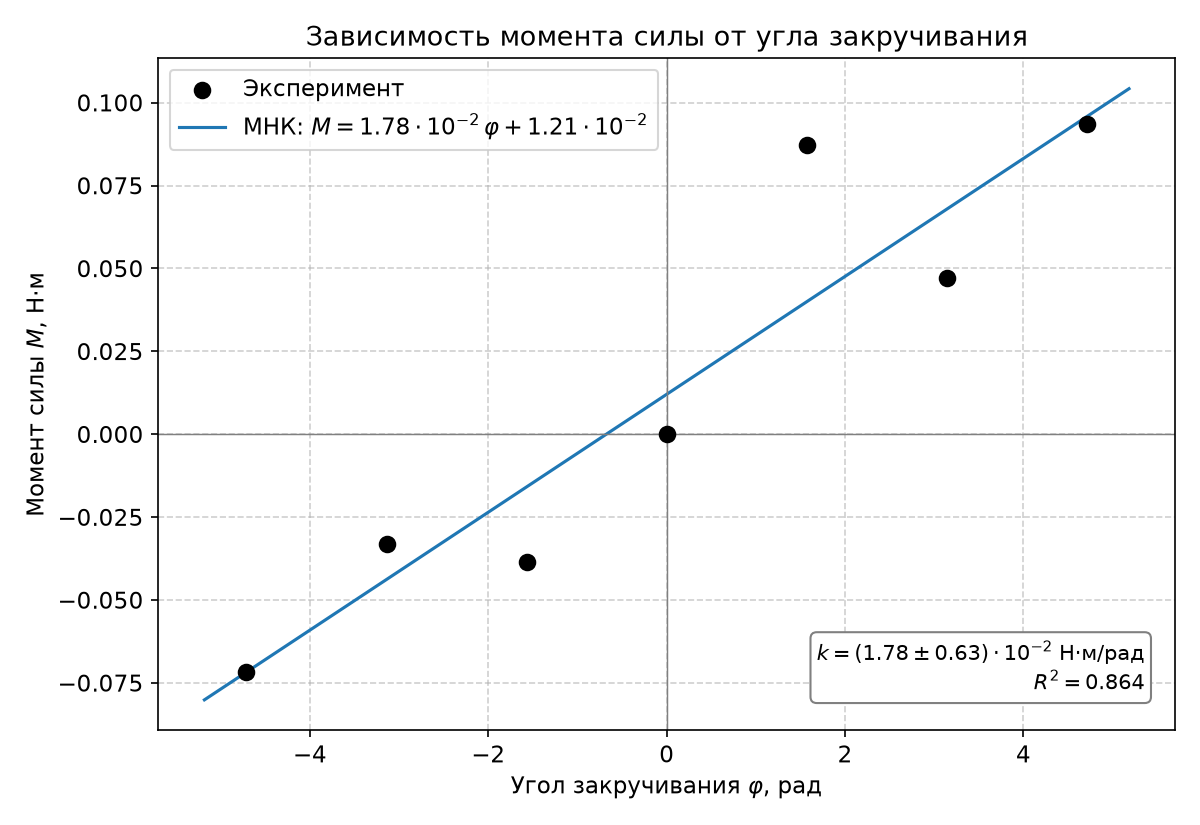
\includegraphics[width=0.85\textwidth]{assets/graph1.png}}
    \caption{Зависимость момента силы от угла закручивания. Точки — эксперимент; линия — МНК: $M = 1.78\cdot10^{-2}\varphi + 1.21\cdot10^{-2}$; $R^2 = 0.86$.}
    \label{fig:graph1}
\end{figure}

\begin{figure}[H]
    \centering
    \fbox{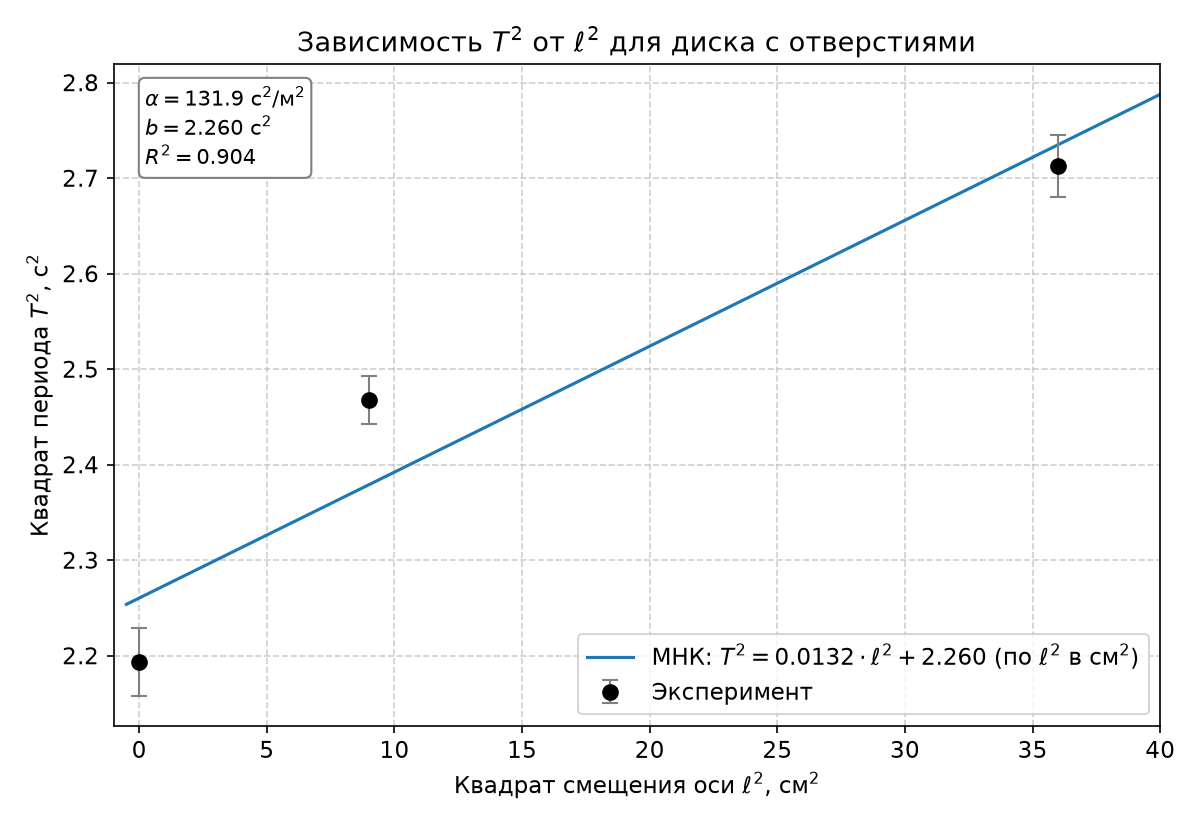
\includegraphics[width=0.85\textwidth]{assets/graph2.png}}
    \caption{Зависимость $T^2$ от $\ell^2$ для диска с отверстиями. Прямая МНК: $T^2 = 132.1\ell^2 + 2.26$.}
    \label{fig:graph2}
\end{figure}

\end{document}